\documentclass{article}

\usepackage{csquotes}
% 使用中文CJK包
\usepackage{CJK}
% 图像插入宏包
\usepackage{graphicx}
% 自定义颜色支持
\usepackage[usenames,dvipsnames]{color}
% 长表格跨页支持
\usepackage{longtable}
% 代码高亮支持
\usepackage{listings}
% 算法伪代码包
\usepackage[ruled,vlined]{algorithm2e}
% 自定义标题格式
\usepackage{titlesec}
% 扩展tabular样式
\usepackage{array}
% 添加页眉页脚
\usepackage{fancyhdr}
% 虚拟正文测试
\usepackage{lipsum}
% 首行缩进
\usepackage{indentfirst}
% 树状结构图
\usepackage{tree-dvips}
% 脚注环境
\usepackage{footnote}
% 定制表格线
\usepackage{makecell}
% tikz绘图包
\usepackage{tikz}
% URL超链接
\usepackage[dvips, colorlinks, linkcolor=black]{hyperref}

% hyperref中文兼容
\pdfstringdefDisableCommands{
\let\CJK@XX\relax
\let\CJK@XXX\relax
\let\CJK@XXXp\relax
\let\CJK@XXXX\relax
\let\CJK@XXXXp\relax
}

\usetikzlibrary{positioning,shapes,shadows,arrows}


% 设置脚注在table中可用
\makesavenoteenv{table}

% 设置标题格式
%\titleformat{\chapter}{\raggedright\Huge\bfseries}{Chapter \thechapter}{1em}{}

% 设置默认字体族, 具体字体请查看texdoc psnfss2e

% 设置Roman字体为Palatino
\renewcommand{\rmdefault}{ppl} 
% 设置TypeWriter字体为Courier
\renewcommand{\ttdefault}{pcr} 

% 设置行距
\setlength{\parskip}{1ex}

% 定义需要的颜色

\definecolor{lightgray}{RGB}{230,230,230}
\definecolor{lightblue}{RGB}{224, 224, 255}
\definecolor{darkblue}{RGB}{192, 192, 255}
\definecolor{lightpink}{RGB}{255, 224, 224}
\definecolor{darkpink}{RGB}{255, 192, 192}
\definecolor{keywordyellow}{RGB}{255, 204, 0}
\definecolor{keywordred}{RGB}{194, 58, 0}
\definecolor{numbercolor}{RGB}{102, 51, 0}

% 设置代码风格

% 定义C语言代码风格
\lstdefinestyle{ccode}
{ 
    language=C, 
    numbers=left, 
    numberstyle=\color{numbercolor},
    basicstyle=\scriptsize\ttfamily\bfseries,
    keywordstyle=\color{blue}, 
    commentstyle=\color{PineGreen},
    stringstyle=\color{red}, 
    frame=shadowbox, 
    frameround=tttt,
    breaklines=true,
    backgroundcolor=\color{lightgray} }

% 定义汇编语言代码风格
\lstdefinestyle{acode}
{ 
    language=,
    morekeywords=[1]{mov, movl, movb, movw, orl, xorw, cli, cld, inb, testb, test, jnz, push, pop, jmp, call, lea, add, sub, ret, jle, outb, ljmp, lgdt},
    morekeywords=[2]{ax, bx, cx, dx, eax, ebx, ecx, edx, cr0, cr1, cr2, cr3, al, ds, es, ss, esp, ebp}, 
    morekeywords=[3]{data, text, bss},
    morekeywords=[4]{long, align, p2align, ascii, fill, globl, space, set, rept, byte, word},
    morecomment=[l]\#,
    numbers=left, 
    numberstyle=\color{numbercolor},
    basicstyle=\scriptsize\ttfamily\bfseries,
    keywordstyle=[1]\color{blue}, 
    keywordstyle=[2]\color{keywordyellow},
    keywordstyle=[3]\color{orange},
    keywordstyle=[4]\color{keywordred},
    commentstyle=\color{PineGreen},
    stringstyle=\color{red}, 
    frame=shadowbox, 
    frameround=tttt,
    breaklines=true,
    backgroundcolor=\color{lightgray} }

    
% 定义命令行输出风格
\lstdefinestyle{console}
{
    language=bash, 
    numbers=none, 
    frame=tRBl,
    basicstyle=\scriptsize\color{green}\ttfamily\bfseries,     
    backgroundcolor=\color{black}}


% 定义exercise输出风格
\lstdefinestyle{exercise}
{
    numbers=none, 
    frame=tRBl,
    breaklines=true,
    breakindent=0pt,
    framexleftmargin=1em,
    framexrightmargin=1em,
    framextopmargin=2ex,
    framexbottommargin=2ex,
    xleftmargin=0.05\linewidth,
    xrightmargin=0.05\linewidth,
    basicstyle=\scriptsize\ttfamily\mdseries,   
    moredelim=[is][\ttfamily\bfseries]{|}{|},
    framerule=0.8pt,
    rulecolor=\color{darkblue}, 
    backgroundcolor=\color{lightblue}}
    

% 定义challenge输出风格
\lstdefinestyle{challenge}
{
    numbers=none, 
    frame=tRBl,
    breaklines=true,
    breakindent=0pt,
    framexleftmargin=1em,
    framexrightmargin=1em,
    framextopmargin=2ex,
    framexbottommargin=2ex,
    xleftmargin=0.05\linewidth,
    xrightmargin=0.05\linewidth,
    basicstyle=\scriptsize\ttfamily\mdseries,   
    moredelim=[is][\ttfamily\bfseries]{|}{|},
    framerule=0.8pt,
    rulecolor=\color{darkpink}, 
    backgroundcolor=\color{lightpink}}
    


% 非常重要, listings关闭非ASCII字符兼容
\lstset{extendedchars=false}


% 定义问题的答案格式
\newcommand{\highlight}[1]{{\bfseries \color{red}  #1}}
% 定义函数名格式
\newcommand{\funcname}[1]{{\ttfamily \small #1}}




\pagestyle{fancy}
\begin{document}
\begin{CJK*}{UTF8}{gkai}

\lhead{操作系统实习报告}
\rhead{张弛, 00848231}
\title{操作系统JOS实习第一次报告}
\author{张弛 \hspace{1ex} 00848231, \\
        zhangchitc@gmail.com}

\maketitle
% 记得在文档末尾插入\clearpage
\tableofcontents
\newpage

\section{PC Bootstrap}

\subsection{Getting Started with x86 assembly}

\begin{lstlisting}[style=exercise]
|Exercise 1|. Familiarize yourself with the assembly language materials available on the 6.828 reference page. You don't have to read them now, but you'll almost certainly want to refer to some of this material when reading and writing x86 assembly.

We do recommend reading the section "The Syntax" in Brennan's Guide to Inline Assembly. It gives a good (and quite brief) description of the AT&T assembly syntax we'll be using with the GNU assembler in JOS.
\end{lstlisting}

Inline 汇编以前从来没有接触过,所以 Brennan's Guide to Inline Assembly 看起来有点陌生,其他的还好。

\subsection{Simulating the x86}

在使用QEMU运行boot loader时,我发现明显的QEMU不如Bochs贴心的一个地方是Bochs提供一条"info gdt"的命令,可以以结构化的方式打印出Global Descriptor Table的基址和各表项,而QEMU却不提供,只有"info registers"可以查看到gdt的基地址,然后利用该地址可以去相应的内存用"xp/xN paddr"查看具体内容。

这个我问了别人好像也是这样。不知道是我们没找到还是QEMU真的就没有?

\subsection{The PC's Physical Address Space}

我本来以为低地址空间0x000A0000 (640KB)之前的空间是不能使用的(为了和老版程序兼容),结果发现在boot loader解压内核的时候,这片Low Memory被用作了临时空间储存内核ELF的文件头。具体来说,ELF文件头被释放到了从地址为0x10000开始的一片4KB空间内。

\subsection{The ROM BIOS}

\begin{lstlisting}[style=exercise]
|Exercise 2|. Use GDB's si (Step Instruction) command to trace into the ROM BIOS for a few more instructions, and try to guess what it might be doing. You might want to look at Phil Storrs I/O Ports Description, as well as other materials on the 6.828 reference materials page. No need to figure out all the details - just the general idea of what the BIOS is doing first.
\end{lstlisting}

IO手册太长了。Orz......

\section{The Boot Loader}

\begin{lstlisting}[style=exercise]
|Exercise 3|. Take a look at the lab tools guide, especially the section on GDB commands. Even if you're familiar with GDB, this includes some esoteric GDB commands that are useful for OS work.

Set a breakpoint at address 0x7c00, which is where the boot sector will be loaded. Continue execution until that breakpoint. Trace through the code in boot/boot.S, using the source code and the disassembly file obj/boot/boot.asm to keep track of where you are. Also use the x/i command in GDB to disassemble sequences of instructions in the boot loader, and compare the original boot loader source code with both the disassembly in obj/boot/boot.asm and GDB.

Trace into bootmain() in boot/main.c, and then into readsect(). Identify the exact assembly instructions that correspond to each of the statements in readsect(). Trace through the rest of readsect() and back out into bootmain(), and identify the begin and end of the for loop that reads the remaining sectors of the kernel from the disk. Find out what code will run when the loop is finished, set a breakpoint there, and continue to that breakpoint. Then step through the remainder of the boot loader.
\end{lstlisting}

Be able to answer the following questions:

\begin{itemize}
\item{At what point does the processor start executing 32-bit code? What exactly causes the switch from 16- to 32-bit mode? }
\item{What is the last instruction of the boot loader executed, and what is the first instruction of the kernel it just loaded? }
\item{Where is the first instruction of the kernel?}
\item{How does the boot loader decide how many sectors it must read in order to fetch the entire kernel from disk? Where does it find this information? }
\end{itemize}

\hrule

\begin{enumerate}
\item{处理器从BIOS进入boot loader后,在boot/boot.S中第48行到第51行代码,\highlight{boot loader将寄存器cr0的末位更改为1,使得处理器从实模式更改到保护模式}。

\begin{lstlisting}[style=acode, firstnumber=44, title={\scriptsize \ttfamily \bfseries boot/boot.S}]
  # Switch from real to protected mode, using a bootstrap GDT
  # and segment translation that makes virtual addresses
  # identical to their physical addresses, so that the
  # effective memory map does not change during the switch.
  lgdt    gdtdesc
  movl    %cr0, %eax
  orl     $CR0_PE_ON, %eax
  movl    %eax, %cr0
\end{lstlisting}
}
\item{\highlight{boot loader执行的最后一条指令为将内核ELF文件载入内存后,调用内核入口点},在boot/main.c中的第58行。
\begin{lstlisting}[style=ccode, firstnumber=56, title={\scriptsize \ttfamily \bfseries boot/main.c}]
    // call the entry point from the ELF header
    // note: does not return!
    ((void (*)(void)) (ELFHDR->e_entry & 0xFFFFFF))();
\end{lstlisting}
}

\item{根据查询objdump -x obj/kern/kernel的结果可以得知内核ELF的入口地址为0xf010000c, 但是boot/main.c在载入内核时做了一次手动的地址转换,将高位的f去掉了,所以事实上在运行中内核是被加载到了0x10000c的内存地址上,所以启动GDB在0x10000c设下断点后,停下时可以看到:

\begin{lstlisting}[style=console]
The target architecture is assumed to be i8086
[f000:fff0]    0xffff0:	ljmp   $0xf000,$0xe05b
0x0000fff0 in ?? ()
+ symbol-file obj/kern/kernel
(gdb) b *0x10000c
Breakpoint 1 at 0x10000c
(gdb) c
Continuing.
The target architecture is assumed to be i386
=> 0x10000c:	movw   $0x1234,0x472

Breakpoint 1, 0x0010000c in ?? ()
(gdb) 
\end{lstlisting}

\highlight{这时0x10000c的代码movw \hspace{1ex}\$0x1234,0x472 就是内核的第一条语句}。这个时候我们反过头来去追溯内核kernel的源代码,果然在kern/entry.S中发现了这么一段代码,其中第44行正好就是我们找到的入口语句。

\begin{lstlisting}[style=acode, firstnumber=36, title={\scriptsize \ttfamily \bfseries kern/entry.S}]
# The Multiboot header
.align 4
.long MULTIBOOT_HEADER_MAGIC
.long MULTIBOOT_HEADER_FLAGS
.long CHECKSUM

.globl      _start
_start:
    movw    $0x1234,0x472           # warm boot

#Establish our own GDT in place of the boot loader's temporary GDT
    lgdt    RELOC(mygdtdesc)        # load descriptor table
\end{lstlisting}
}

\item{\highlight{boot loader从内核ELF文件的文件头中可以知道该ELF文件被分成了多少section和多少program},就可以知道相应的读取数目了。这些信息可以通过objdump -x obj/kern/kernel得到,如下所示:
\begin{lstlisting}[style=console]
zhangchi@zhangchi-laptop:~/oslab$ objdump -x obj/kern/kernel

obj/kern/kernel:     file format elf32-i386
obj/kern/kernel
architecture: i386, flags 0x00000112:
EXEC_P, HAS_SYMS, D_PAGED
start address 0xf010000c

Program Header:
    LOAD off    0x00001000 vaddr 0xf0100000 paddr 0xf0100000 align 2**12
         filesz 0x000072e7 memsz 0x000072e7 flags r-x
    LOAD off    0x00009000 vaddr 0xf0108000 paddr 0xf0108000 align 2**12
         filesz 0x00008320 memsz 0x00008980 flags rw-
   STACK off    0x00000000 vaddr 0x00000000 paddr 0x00000000 align 2**2
         filesz 0x00000000 memsz 0x00000000 flags rwx

\end{lstlisting}
}
\end{enumerate}

\subsection{Loading the Kernel}

\begin{lstlisting}[style=exercise]
|Exercise 4|. Read about programming with pointers in C. The best reference for the C language is The C Programming Language by Brian Kernighan and Dennis Ritchie (known as 'K&R'). We recommend that students purchase this book (here is an Amazon Link) or find one of MIT's 7 copies.

Read 5.1 (Pointers and Addresses) through 5.5 (Character Pointers and Functions) in K&R. Then download the code for pointers.c, run it, and make sure you understand where all of the printed values come from. In particular, make sure you understand where the pointer addresses in lines 1 and 6 come from, how all the values in lines 2 through 4 get there, and why the values printed in line 5 are seemingly corrupted.

There are other references on pointers in C, though not as strongly recommended. A tutorial by Ted Jensen that cites K&R heavily is available in the course readings.

Warning: Unless you are already thoroughly versed in C, do not skip or even skim this reading exercise. If you do not really understand pointers in C, you will suffer untold pain and misery in subsequent labs, and then eventually come to understand them the hard way. Trust us; you don't want to find out what "the hard way" is.
\end{lstlisting}

pointers.c里只有一句比较不好解释:

\begin{lstlisting}[style=ccode, numbers=none]
    c = (int *) ((char *) c + 1);
    *c = 500;
\end{lstlisting}

其中c修改的是一个int从第九位开始到第32位,然后将后面一个数的低8位覆盖。所以造成的结果很奇怪,不过手动还是可以精确算出来结果的。

\vspace{3em}

\begin{lstlisting}[style=exercise]
|Exercise 5|. Reset the machine (exit QEMU/GDB and start them again). Examine the 8 words of memory at 0x00100000 at the point the BIOS enters the boot loader, and then again at the point the boot loader enters the kernel. Why are they different? What is there at the second breakpoint? (You do not really need to use QEMU to answer this question. Just think.)
\end{lstlisting}

经过调试我们得到了GDB这样的输出:

\begin{lstlisting}[style=console]
The target architecture is assumed to be i8086
[f000:fff0]    0xffff0:	ljmp   $0xf000,$0xe05b
0x0000fff0 in ?? ()
+ symbol-file obj/kern/kernel
(gdb) b *0x7c00
Breakpoint 1 at 0x7c00
(gdb) c
Continuing.
[   0:7c00] => 0x7c00:	cli    

Breakpoint 1, 0x00007c00 in ?? ()
(gdb) x/8x 0x100000
0x100000:	0x00000000	0x00000000	0x00000000	0x00000000
0x100010:	0x00000000	0x00000000	0x00000000	0x00000000
(gdb) b *0x10000c
Breakpoint 2 at 0x10000c
(gdb) c
Continuing.
The target architecture is assumed to be i386
=> 0x10000c:	movw   $0x1234,0x472

Breakpoint 2, 0x0010000c in ?? ()
(gdb) x/8x 0x100000
0x100000:	0x1badb002	0x00000003	0xe4524ffb	0x7205c766
0x100010:	0x34000004	0x15010f12	0x00110018	0x000010b8
(gdb) x/8i 0x100000
   0x100000:	add    0x31bad(%eax),%dh
   0x100006:	add    %al,(%eax)
   0x100008:	sti    
   0x100009:	dec    %edi
   0x10000a:	push   %edx
   0x10000b:	in     $0x66,%al
   0x10000d:	movl   $0x10f1234,0x472
   0x100017:	adc    $0x110018,%eax
(gdb) 

\end{lstlisting}

内存0x00100000是内核的最终载入地址,内核由Boot loader负责载入。初始当BIOS切换到boot loader时,它还没有开始相应的装载工作,所以这个时候看所有的8个word全是0。而当boot loader进入内核运行时,这个时候内核已经装载完毕,所以从0x00100000开始就是内核ELF文件的文件内容了。

\subsection{Link vs. Load Address}

\begin{lstlisting}[style=exercise]
|Exercise 6|. Trace through the first few instructions of the boot loader again and identify the first instruction that would "break" or otherwise do the wrong thing if you were to get the boot loader's link address wrong. Then change the link address in boot/Makefrag to something wrong, run make clean, recompile the lab with make, and trace into the boot loader again to see what happens. Don't forget to change the link address back and make clean again afterward!
\end{lstlisting}

我把boot/Makefrag中第28行-Ttext参数从0x7c00改成了0x7c04,即实际的boot loader装载位置比链接位置要后,我们看看重新编译启动的效果:

\begin{lstlisting}[style=console]
The target architecture is assumed to be i8086
[f000:fff0]    0xffff0:	ljmp   $0xf000,$0xe05b
0x0000fff0 in ?? ()
+ symbol-file obj/kern/kernel
(gdb) c
Continuing.

Program received signal SIGTRAP, Trace/breakpoint trap.
[   0:7c2d] => 0x7c2d:	ljmp   $0x8,$0x7c36
0x00007c2d in ?? ()
(gdb) 
\end{lstlisting}

可以看到在0x7c2d:\hspace{1ex} ljmp \hspace{0.5ex} \$0x8,\$0x7c36这条代码上运行出错,这条代码位于boot/boot.S中第55行,我们把boot/boot.S从开始到这行的所有代码列出:

\begin{lstlisting}[style=acode, firstnumber=12, title={\scriptsize \ttfamily \bfseries boot/boot.S}]
.globl start
start:
  .code16                     # Assemble for 16-bit mode
  cli                         # Disable interrupts
  cld                         # String operations increment

  # Set up the important data segment registers (DS, ES, SS).
  xorw    %ax,%ax             # Segment number zero
  movw    %ax,%ds             # -> Data Segment
  movw    %ax,%es             # -> Extra Segment
  movw    %ax,%ss             # -> Stack Segment

  # Enable A20:
  #   For backwards compatibility with the earliest PCs, physical
  #   address line 20 is tied low, so that addresses higher than
  #   1MB wrap around to zero by default.  This code undoes this.
seta20.1:
  inb     $0x64,%al               # Wait for not busy
  testb   $0x2,%al
  jnz     seta20.1

  movb    $0xd1,%al               # 0xd1 -> port 0x64
  outb    %al,$0x64

seta20.2:
  inb     $0x64,%al               # Wait for not busy
  testb   $0x2,%al
  jnz     seta20.2

  movb    $0xdf,%al               # 0xdf -> port 0x60
  outb    %al,$0x60

  # Switch from real to protected mode, using a bootstrap GDT
  # and segment translation that makes virtual addresses 
  # identical to their physical addresses, so that the 
  # effective memory map does not change during the switch.
  lgdt    gdtdesc
  movl    %cr0, %eax
  orl     $CR0_PE_ON, %eax
  movl    %eax, %cr0
  
  # Jump to next instruction, but in 32-bit code segment.
  # Switches processor into 32-bit mode.
  ljmp    $PROT_MODE_CSEG, $protcseg

  .code32                     # Assemble for 32-bit mode
\end{lstlisting}

很明显,\highlight{只有涉及相对位置跳转的语句才有可能在链接地址和装载地址不一致的时候发生问题},如

\begin{lstlisting}[style=acode, firstnumber=31]
  jnz     seta20.1
\end{lstlisting}

和

\begin{lstlisting}[style=acode, firstnumber=39]
  jnz     seta20.2
\end{lstlisting}

以及

\begin{lstlisting}[style=acode, firstnumber=55]
  ljmp    $PROT_MODE_CSEG, $protcseg
\end{lstlisting}

最终是第55行的代码出错,这是因为前面两句都是进行设备的忙等待的轮询语句,很可能是设备在其一开始检测的时候就准备好了,所以条件跳转无效。而55行语句是切换到32位保护模式后进行设备初始化的工作,是一定会跳转的。所以执行到这里就出错了。


\section{The Kernel}

\begin{lstlisting}[style=exercise]
|Exercise 7|. Use QEMU and GDB to trace into the JOS kernel and find where the new virtual-to-physical mapping takes effect. Then examine the Global Descriptor Table (GDT) that the code uses to achieve this effect, and make sure you understand what's going on.

What is the first instruction after the new mapping is established that would fail to work properly if the old mapping were still in place? Comment out or otherwise intentionally break the segmentation setup code in kern/entry.S, trace into it, and see if you were right.
\end{lstlisting}

boot loader在进行初始化数据的时候自己定义了GDT,切换到内核运行后,内核在载入初期马上重新定义了自己的GDT,然后替换掉了原有的GDT,从代码kern/entry.S可以看到

\begin{lstlisting}[style=acode, firstnumber=42, title={\scriptsize \ttfamily \bfseries kern/entry.S}]
.globl      _start
_start:
    movw    $0x1234,0x472           # warm boot

    # Establish our own GDT in place of the boot loader's temporary GDT.
    lgdt    RELOC(mygdtdesc)        # load descriptor table

    # Immediately reload all segment registers (including CS!)
    # with segment selectors from the new GDT.
    movl    $DATA_SEL, %eax         # Data segment selector
    movw    %ax,%ds             # -> DS: Data Segment
    movw    %ax,%es             # -> ES: Extra Segment
    movw    %ax,%ss             # -> SS: Stack Segment
    ljmp    $CODE_SEL,$relocated        # reload CS by jumping
relocated:

    # Clear the frame pointer register (EBP)
    # so that once we get into debugging C code,
    # stack backtraces will be terminated properly.
    movl    $0x0,%ebp           # nuke frame pointer

    # Set the stack pointer
    movl    $(bootstacktop),%esp

    # now to C code
    call    i386_init
\end{lstlisting}

在进入内核以后第47行代码,内核就启用了新的GDT,找到其定义所在的mygdtdesc:

\begin{lstlisting}[style=acode, firstnumber=93, title={\scriptsize \ttfamily \bfseries kern/entry.S}]
###################################################################
# setup the GDT 
###################################################################
    .p2align    2       # force 4 byte alignment
mygdt:
    SEG_NULL                # null seg
    SEG(STA_X|STA_R, -KERNBASE, 0xffffffff) # code seg
    SEG(STA_W, -KERNBASE, 0xffffffff)   # data seg
mygdtdesc:
    .word   0x17            # sizeof(mygdt) - 1
    .long   RELOC(mygdt)        # address mygdt
\end{lstlisting}

可以看到新的描述表和原来的不同了,新的段表其基址全部变成了-KERNBASE而不是原来的0,通过查找定义在inc/memlayout.h中的KERNBASE定义:

\begin{lstlisting}[style=ccode, firstnumber=81, title={\scriptsize \ttfamily \bfseries inc/memlayout.h}]
// All physical memory mapped at this address
#define KERNBASE    0xF0000000
\end{lstlisting}

可以看到每次相对寻址时-KERNBASE如果和内核的链接地址0xf01xxxxx相加的话,就自动将最高的f去掉了,这个和boot loader的boot/main.c在载入内核ELF的分段时使用的与地址法在效果上是完全一致的。下面的代码是 main.c在 readseg 时使用的具体地址转换机制。

\begin{lstlisting}[style=ccode, firstnumber=67, title={\scriptsize \ttfamily \bfseries boot/main.c}]
// Read 'count' bytes at 'offset' from kernel into virtual address 'va'.
// Might copy more than asked
void
readseg(uint32_t va, uint32_t count, uint32_t offset)
{
    uint32_t end_va;

    va &= 0xFFFFFF;
    end_va = va + count;

    // round down to sector boundary
    va &= ~(SECTSIZE - 1);
\end{lstlisting}


为了验证我的想法,我尝试着注释掉了kern/entry.S中的第47行启用新GDT的代码,然后编译后重启启动JOS,GDB给出了这样的错误信息:

\begin{lstlisting}[style=console]
The target architecture is assumed to be i8086
[f000:fff0]    0xffff0:	ljmp   $0xf000,$0xe05b
0x0000fff0 in ?? ()
+ symbol-file obj/kern/kernel
(gdb) c
Continuing.

Program received signal SIGTRAP, Trace/breakpoint trap.
The target architecture is assumed to be i386
=> 0xf0100027 <relocated>:	(bad)  
relocated () at kern/entry.S:61
61		movl	$0x0,%ebp			# nuke frame pointer
(gdb) 
\end{lstlisting}

想法得到了验证,GDB在运行到0xf0100027时,指针寻址发生了错误。

\subsection{Formatted Printing to the Console}

\begin{lstlisting}[style=exercise]
|Exercise 8|. We have omitted a small fragment of code - the code necessary to print octal numbers using patterns of the form "%o". Find and fill in this code fragment.
\end{lstlisting}

Be able to answer the following questions:

\begin{enumerate}
\item{Explain the interface between printf.c and console.c. Specifically, what function does console.c export? How is this function used by printf.c?}
\item{Explain the following from console.c:
{\scriptsize
\begin{verbatim}
if (crt_pos >= CRT_SIZE) {
       int i;
       memcpy(crt_buf, crt_buf + CRT_COLS, (CRT_SIZE - CRT_COLS) * sizeof(uint16_t));
       for (i = CRT_SIZE - CRT_COLS; i < CRT_SIZE; i++)
             crt_buf[i] = 0x0700 | ' ';
       crt_pos -= CRT_COLS;
}
\end{verbatim}}
}
\item{For the following questions you might wish to consult the notes for Lecture 2. These notes cover GCC's calling convention on the x86.

Trace the execution of the following code step-by-step:
{\scriptsize
\begin{verbatim}
int x = 1, y = 3, z = 4;
cprintf("x %d, y %x, z %d\n", x, y, z);
\end{verbatim}}

\begin{itemize}
\item{In the call to \funcname{cprintf()}, to what does \funcname{fmt} point? To what does \funcname{ap} point?}
\item{List (in order of execution) each call to \funcname{cons\_putc, va\_arg}, and \funcname{vcprintf}. For \funcname{cons\_putc}, list its argument as well. For \funcname{va\_arg}, list what ap points to before and after the call. For \funcname{vcprintf} list the values of its two arguments.}
\end{itemize}
}
\item{Run the following code.

{\scriptsize
\begin{verbatim}
    unsigned int i = 0x00646c72;
    cprintf("H%x Wo%s", 57616, &i);
\end{verbatim}}
What is the output? Explain how this output is arrived at in the step-by-step manner of the previous exercise. Here's an ASCII table that maps bytes to characters.

The output depends on that fact that the x86 is little-endian. If the x86 were instead big-endian what would you set i to in order to yield the same output? Would you need to change 57616 to a different value?

Here's a description of little- and big-endian and a more whimsical description.
}
\item{
In the following code, what is going to be printed after '\funcname{y=}'? (note: the answer is not a specific value.) Why does this happen?
{\scriptsize
\begin{verbatim}
    cprintf("x=%d y=%d", 3);
\end{verbatim}}
}
\item{Let's say that GCC changed its calling convention so that it pushed arguments on the stack in declaration order, so that the last argument is pushed last. How would you have to change \funcname{cprintf} or its interface so that it would still be possible to pass it a variable number of arguments?}
\end{enumerate}

\hrule
\vspace{2em}

关于lib/printfmt.c中八进制打印的实现,非常简单,只要把原来的:

\begin{lstlisting}[style=ccode, firstnumber=207, title={\scriptsize \ttfamily \bfseries lib/printfmt.c}]
        // (unsigned) octal
        case 'o':
            // Replace this with your code.
            putch('X', putdat);
            putch('X', putdat);
            putch('X', putdat);
            break;
\end{lstlisting}

替换成

\begin{lstlisting}[style=ccode, firstnumber=207, title={\scriptsize \ttfamily \bfseries lib/printfmt.c}]
        // (unsigned) octal
        case 'o':
            num = getuint(&ap, lflag);
            base = 8;

            goto number;
\end{lstlisting}

\vspace{2em}
\hrule
\vspace{2em}

\begin{enumerate}
\item{kern/console.c主要提供一些与硬件直接进行交互的接口以便其他程序进行输入输出的调用。其中与kern/printf.c进行交互的主要是\funcname{cputchar} 函数。

\begin{lstlisting}[style=ccode, firstnumber=455, title={\scriptsize \ttfamily \bfseries kern/console.c}]
// `High'-level console I/O.  Used by readline and cprintf.

void
cputchar(int c)
{
	cons_putc(c);
}
\end{lstlisting}

该函数用于将一个字符输出到显示器。在kern/printf.c中被 \funcname{putch} 调用

\begin{lstlisting}[style=ccode, firstnumber=9, title={\scriptsize \ttfamily \bfseries kern/printf.c}]
static void
putch(int ch, int *cnt)
{
	cputchar(ch);
	*cnt++;
}
\end{lstlisting}

}
\item{
\begin{lstlisting}[style=ccode, firstnumber=194, title={\scriptsize \ttfamily \bfseries kern/console.c}]
if (crt_pos >= CRT_SIZE) {
       int i;
       memcpy(crt_buf, crt_buf + CRT_COLS, (CRT_SIZE - CRT_COLS) * sizeof(uint16_t));
       for (i = CRT_SIZE - CRT_COLS; i < CRT_SIZE; i++)
             crt_buf[i] = 0x0700 | ' ';
       crt_pos -= CRT_COLS;
}
\end{lstlisting}

上面这段代码主要用于在打印后检测是否满屏,如果满屏,则将最后一行空出来,全部置为空格,而最上一行则被抛弃。同时将光标置于最后一行的行首。
}

\item{
\begin{itemize}
\item{ 在 \funcname{cprintf()}中, \funcname{fmt}指向的是格式字符串,在上例中即\funcname{"x \%d, y \%x, z \%d \textbackslash n"},而\funcname{ap}指向的是不定参数表的第一个参数地址,在上例中即x}
\item{具体调试信息太长,这里就不贴了。\funcname{va\_arg}的作用是将ap每次指向的地址往后移动需要的类型个字节。}
\end{itemize}
}
\item{打印出的内容是
\begin{lstlisting}[style=console]
Welcome to the JOS kernel monitor!
Type 'help' for a list of commands.
He110 World
K> 
\end{lstlisting}

这是因为57616的16进制表示就是e11,而unsigned \hspace{0.5ex} int \hspace{1ex} 0x00646c72在little endian的机器上用char*表示出来就是\{0x72, 0x6c, 0x64, 0x00\} = \{'r', 'l', 'd', '\textbackslash 0'\}

如果在big endian机器上想要打印出"He110 World"的话,i的值必须改为0x726c6400,而e110的打印则和57616的具体储存方式没有关系,可以不用更改。

}
\item{打印出的结果为

\begin{lstlisting}[style=console]
Welcome to the JOS kernel monitor!
Type 'help' for a list of commands.
x=3 y=-267380146
K> 
\end{lstlisting}

因为根据\funcname{vprintfmt} 的机制,每次打印的变量值都是根据va\_arg从ap指针不断的往后取得到的。如果给的参数数量不足实际要打印的数量,那么最后ap就跳到了一个未知内存区域,所以打印出来的东西很奇怪。

}
\item{ 具体变长参数依赖于inc/stdarg.h中\funcname{va\_arg}的实现。
\begin{lstlisting}[style=ccode, title={\scriptsize \ttfamily \bfseries inc/stdarg.h}]
/*	$NetBSD: stdarg.h,v 1.12 1995/12/25 23:15:31 mycroft Exp $	*/

#ifndef JOS_INC_STDARG_H
#define	JOS_INC_STDARG_H

typedef char *va_list;

#define	__va_size(type) \
	(((sizeof(type) + sizeof(long) - 1) / sizeof(long)) * sizeof(long))

#define	va_start(ap, last) \
	((ap) = (va_list)&(last) + __va_size(last))

#define	va_arg(ap, type) \
	(*(type *)((ap) += __va_size(type), (ap) - __va_size(type)))

#define	va_end(ap)	((void)0)

#endif	/* !JOS_INC_STDARG_H */
\end{lstlisting}

从上面可以看到,\funcname{va\_arg} 每次是以地址往后增长取出下一参数变量的地址的。而这个实现方式就\highlight{默认假设了编译器是以从右往左的顺序将参数入栈的}。因为栈是以从高往低的方向增长的。后压栈的参数放在了内存地址的低位置,所以如果要以从左到右的顺序依次取出每个变量,那么编译器必须以相反的顺序即从右往左将参数压栈。

如果编译器更改了压栈的顺序,那么为了仍然能正确取出所有的参数,那么需要修改上面代码中的\funcname{va\_start}和\funcname{va\_arg}两个宏,将其改成用减法得到新地址即可。
}
\end{enumerate}

\vspace{2em}

\begin{lstlisting}[style=challenge]
|Challenge| Enhance the console to allow text to be printed in different colors. The traditional way to do this is to make it interpret ANSI escape sequences embedded in the text strings printed to the console, but you may use any mechanism you like. There is plenty of information on the 6.828 reference page and elsewhere on the web on programming the VGA display hardware. If you're feeling really adventurous, you could try switching the VGA hardware into a graphics mode and making the console draw text onto the graphical frame buffer.
\end{lstlisting}

首先其实JOS是提供了颜色打印的功能的,追溯一个字符的打印过程,其实是从\funcname{cprintf} $\rightarrow$ \funcname{vcprintf} $\rightarrow$ \funcname{vprintfmt} $\rightarrow$ \funcname{putch} $\rightarrow$ \funcname{cputchar} $\rightarrow$ \funcname{cons\_putc} $\rightarrow$ \funcname{cga\_putc}这样的调用路径,最后在\funcname{cga\_putc}中,我们可以看到关于颜色控制的相关机制:

\begin{lstlisting}[style=ccode, firstnumber=164, title={\scriptsize \ttfamily \bfseries kern/console.c}]
static void
cga_putc(int c)
{
	// if no attribute given, then use black on white
	if (!(c & ~0xFF))
		c |= 0x0700;
\end{lstlisting}

在c参数中,低8位是为了指定需要打印的字符的ASCII码,而高八位则是指定打印的颜色。可以看到代码中如果不设置颜色则默认是黑底白字,高八位为07。其高8位具体含义如下:

\begin{table}[htp]
\centering
\makegapedcells
\setcellgapes{5pt}

\begin{tabular}{
!{\vrule width2pt} c
!{\vrule width2pt} c
!{\vrule width2pt} c
!{\vrule width2pt} c
!{\vrule width2pt} c
!{\vrule width2pt} c
!{\vrule width2pt} c
!{\vrule width2pt} c
!{\vrule width2pt}}
15 & 14 & 13 & 12 & 11 & 10 & 9 & 8 \\
\Xhline{2pt}
B\_I & B\_R & B\_G & B\_B & F\_I & F\_R & F\_G & F\_B \\
\Xhline{2pt}
\end{tabular}
\end{table}

c的15到12位用于指定字符的背景颜色,颜色由3位RGB颜色代码+I味是否高亮指定。11到8位用于指定字符的前景颜色。

搞清楚打印的原理以后,我决定仿照类似ANSI的颜色控制字的思想来构造彩色打印机制。

\begin{itemize}
    \item{在\funcname{cprintf}的格式字符串中增加格式化参数\%C,用来指定从这个参数以后打印的所有字符颜色,那么直到碰到下一个格式化参数\%C,这之间的所有参数都将会由\%C指定的颜色打出}
    \item{\%C出现后后接三位数字用于指定具体颜色,表示8位颜色指定码,所以三位数字需要在0到255之间,而且如果不到3位数的话,需要添加前导0}
    \item{为了方便常用颜色的使用,定义一组三位字符为颜色指定符,用于代替数字,可以直观的使用}
\end{itemize}

确定了控制机制以后,我们需要考虑如何在代码实现控制的接口。发出打印命令是在\funcname{cprintf}函数中,按照调用链条到达\funcname{vprintfmt}开始分析格式控制字符,然后在\funcname{cga\_putc}中实现打印具体字符。这样来看我们是在\funcname{vprintfmt}函数中捕捉到颜色控制命令以后,要传递给\funcname{cga\_putc}函数。可以直接在\funcname{vprintfmt}中所有调用\funcname{putch}函数时将传入的字符添加上高位颜色信息。但是这样太麻烦了,因为\funcname{vprintfmt}中有十几个直接调用\funcname{putch}的地方,还有间接调用,比如\funcname{vprintfmt} $\rightarrow$ \funcname{printnum} $\rightarrow$ \funcname{putch},这样所有的地方都要改,难免出错。

所以我选择了一个牺牲封闭性,但简洁易行的方法。就是在\funcname{vprintfmt}中定义一个全局变量ch\_color,每次遇到一个颜色指令后,就修改它,然后在\funcname{cga\_putc}中用extern指令引用这个全局变量,打印时直接将这个颜色信息加入打印字符中。这样修改起来就非常方便了。

具体实施起来,先对kern/console.c的\funcname{cga\_putc}进行一下小的修改,修改为:

\begin{lstlisting}[style=ccode, title={\scriptsize \ttfamily \bfseries kern/console.c}]
extern int ch_color;

static void
cga_putc(int c)
{
        c = c + (ch_color << 8);

	// if no attribute given, then use black on white
	if (!(c & ~0xFF))
		c |= 0x0700;
\end{lstlisting}

对于lib/printfmt.c,首先先定义一些特定的常用颜色:


\begin{lstlisting}[style=ccode, title={\scriptsize \ttfamily \bfseries lib/printfmt.c}]
#define COLOR_WHT 7;
#define COLOR_BLK 1;
#define COLOR_GRN 2;
#define COLOR_RED 4;
#define COLOR_GRY 8;
#define COLOR_YLW 15;
#define COLOR_ORG 12;
#define COLOR_PUR 6;
#define COLOR_CYN 11;

int ch_color = COLOR_WHT;
\end{lstlisting}

颜色码为高8位的具体数值。然后就可以在\funcname{vprintfmt}函数里添加具体的解析模块了,如下代码:

\begin{lstlisting}[style=ccode, firstnumber=172, title={\scriptsize \ttfamily \bfseries lib/printfmt.c}]
        // character
        case 'c':
            putch(va_arg(ap, int), putdat);
            break;


        // color control
        case 'C':
            // void* memmove (void *dst, const void *src, size_t len) 
            // was declared in inc/string.h
            // it could be used to replace memcpy ()

            memmove (sel_c, fmt, sizeof(unsigned char) * 3);
            sel_c[3] = '\0';
            fmt += 3;

            if (sel_c[0] >= '0' && sel_c[0] <= '9') {
                // it is a color specifier
                // JOS provide no atoi, we can only convert char* all by ourselves
           
                ch_color = ((sel_c[0] - '0') * 10 + sel_c[1] - '0') * 10 + sel_c[2] - '0';

            } else {
                // it is a explicit color selector
                
                // strcmp (const char *s1, const char *s2) 
                // was declared in inc/string.h
                if (strcmp (sel_c, "wht") == 0) ch_color = COLOR_WHT else
                if (strcmp (sel_c, "blk") == 0) ch_color = COLOR_BLK else
                if (strcmp (sel_c, "grn") == 0) ch_color = COLOR_GRN else
                if (strcmp (sel_c, "red") == 0) ch_color = COLOR_RED else
                if (strcmp (sel_c, "gry") == 0) ch_color = COLOR_GRY else
                if (strcmp (sel_c, "ylw") == 0) ch_color = COLOR_YLW else
                if (strcmp (sel_c, "org") == 0) ch_color = COLOR_ORG else
                if (strcmp (sel_c, "pur") == 0) ch_color = COLOR_PUR else
                if (strcmp (sel_c, "cyn") == 0) ch_color = COLOR_CYN else
                    ch_color = COLOR_WHT;
            }
            break;
\end{lstlisting}

这样打印的具体工作就完成了,测试一下,我把在kern/monitor.c中打印欢迎信息的语句替换成了现在这样:

\begin{lstlisting}[style=ccode, title={\scriptsize \ttfamily \bfseries kern/monitor.c}]
void
monitor(struct Trapframe *tf)
{
  char *buf;

  cprintf("%CredWelcome %Cwhtto %Cgrnthe %CorgJOS %Cgrykernel %Cpurmonitor!\n");
  cprintf("%CcynType %Cylw'help' %C142for a %C201list %C088of %Cwhtcommands.\n");
\end{lstlisting}

那么启动后系统打印出的信息如图所示!!!!

\begin{figure}[htp]
\centering
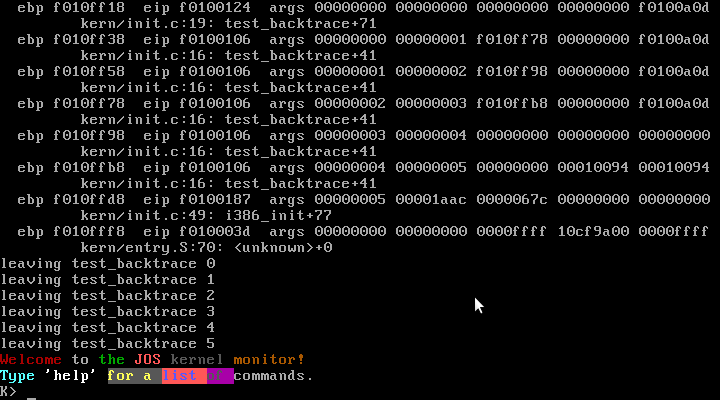
\includegraphics[scale=0.40]{/home/zhangchi/codezhangchitc/Homework/Junior_II/OS/rep1/screenshot.png}
\end{figure}

\subsection{The Stack}

\begin{lstlisting}[style=exercise]
|Exercise 9|. Determine where the kernel initializes its stack, and exactly where in memory its stack is located. How does the kernel reserve space for its stack? And at which "end" of this reserved area is the stack pointer initialized to point to?
\end{lstlisting}

内核进行栈初始化的代码段位于kern/entry.S中,如下列代码

\begin{lstlisting}[style=acode, firstnumber=56, title={\scriptsize \ttfamily \bfseries kern/entry.S}]
relocated:

	# Clear the frame pointer register (EBP)
	# so that once we get into debugging C code,
	# stack backtraces will be terminated properly.
	movl	$0x0,%ebp			# nuke frame pointer

	# Set the stack pointer
	movl	$(bootstacktop),%esp

	# now to C code
	call	i386_init
\end{lstlisting}

内核初始作的工作主要是将寄存器\%ebp初始为0,\%esp初始化为bootstacktop,我们进入bootstacktop的定义位置进行查看:

\begin{lstlisting}[style=acode, firstnumber=83, title={\scriptsize \ttfamily \bfseries kern/entry.S}]
###################################################################
# boot stack
###################################################################
	.p2align	PGSHIFT		# force page alignment
	.globl		bootstack
bootstack:
	.space		KSTKSIZE
	.globl		bootstacktop   
bootstacktop:
\end{lstlisting}

栈的空间定义在ELF文件中的.data段,载入内核时根据data段在ELF文件中的相对位置被载入内存。

我们发现栈有两部分,第一部分是实际栈空间,一共KSTKSIZE,其大小定义在inc/memlayout.h中, $\mbox{KSTKSIZE} = 8 \times \mbox{PGSIZE} = 8 \times 4096\mbox{B} = 32\mbox{KB}$,另一部分是栈底指针bootstacktop,因为它指向栈空间定义完以后的高地址位置。前面我们说过栈是向低地址生长的,所以最高位置就是栈底。这个位置最终会作为初值传递给\%esp。

\vspace{4em}

\begin{lstlisting}[style=exercise]
|Exercise 10|. To become familiar with the C calling conventions on the x86, find the address of the test_backtrace function in obj/kern/kernel.asm, set a breakpoint there, and examine what happens each time it gets called after the kernel starts. How many 32-bit words does each recursive nesting level of test_backtrace push on the stack, and what are those words?

Note that, for this exercise to work properly, you should be using the patched version of QEMU available on the tools page or on Athena. Otherwise, you'll have to manually translate all breakpoint and memory addresses to linear addresses.
\end{lstlisting}

首先我们来观察一下obj/kern/kernel.asm中\funcname{test\_backtrace}的汇编代码到底是怎样做的:

\begin{lstlisting}[style=acode, firstnumber=150, title={\scriptsize \ttfamily \bfseries obj/kern/kernel.asm}]
// Test the stack backtrace function (lab 1 only)
void
test_backtrace(int x)
{
f01000dd:	55                   	push   %ebp
f01000de:	89 e5                	mov    %esp,%ebp
f01000e0:	53                   	push   %ebx
f01000e1:	83 ec 14             	sub    $0x14,%esp
f01000e4:	8b 5d 08             	mov    0x8(%ebp),%ebx
	cprintf("entering test_backtrace %d\n", x);
f01000e7:	89 5c 24 04          	mov    %ebx,0x4(%esp)
f01000eb:	c7 04 24 12 1a 10 f0 	movl   $0xf0101a12,(%esp)
f01000f2:	e8 34 08 00 00       	call   f010092b <cprintf>
	if (x > 0)
f01000f7:	85 db                	test   %ebx,%ebx
f01000f9:	7e 0d                	jle    f0100108 <test_backtrace+0x2b>
		test_backtrace(x-1);
f01000fb:	8d 43 ff             	lea    -0x1(%ebx),%eax
f01000fe:	89 04 24             	mov    %eax,(%esp)
f0100101:	e8 d7 ff ff ff       	call   f01000dd <test_backtrace>
f0100106:	eb 1c                	jmp    f0100124 <test_backtrace+0x47>
	else
		mon_backtrace(0, 0, 0);
f0100108:	c7 44 24 08 00 00 00 	movl   $0x0,0x8(%esp)
f010010f:	00 
f0100110:	c7 44 24 04 00 00 00 	movl   $0x0,0x4(%esp)
f0100117:	00 
f0100118:	c7 04 24 00 00 00 00 	movl   $0x0,(%esp)
f010011f:	e8 7c 05 00 00       	call   f01006a0 <mon_backtrace>
	cprintf("leaving test_backtrace %d\n", x);
f0100124:	89 5c 24 04          	mov    %ebx,0x4(%esp)
f0100128:	c7 04 24 2e 1a 10 f0 	movl   $0xf0101a2e,(%esp)
f010012f:	e8 f7 07 00 00       	call   f010092b <cprintf>
}
f0100134:	83 c4 14             	add    $0x14,%esp
f0100137:	5b                   	pop    %ebx
f0100138:	5d                   	pop    %ebp
f0100139:	c3                   	ret    
\end{lstlisting}

可以看到,一共有四类栈空间被使用
\begin{itemize}
\item{入口处按照C \hspace{1ex}Convention将\%ebp保存使用的栈空间}
\item{第156行,还在栈里保存了\%ebx,通过后面的代码可以看到该函数使用到了\%ebx通用寄存器,所以156行的作用是保存现场3以便退出时恢复}
\item{第157行,函数保留了0x14个即20个byte的空间作为临时变量储存,包括在作为caller调用其他函数时,给该函数(callee)的参数,也放在这20 byte的空间中,通过第158行可以看出,参数x的值存放在0x8(\%ebp)即原来备份\%ebp寄存器上面的位置}
\item{第169行,assembler在进行call命令执行时,会自动将\%eip的值压入栈中}
\end{itemize}

综上,每次调用,一共会有$4 + 4 + 20 + 4 = 32$byte的空间会被压入栈中。

\vspace{4em}

\begin{lstlisting}[style=exercise]
|Exercise 11|. Implement the backtrace function as specified above. Use the same format as in the example, since otherwise the grading script will be confused. When you think you have it working right, run make grade to see if its output conforms to what our grading script expects, and fix it if it doesn't. After you have handed in your Lab 1 code, you are welcome to change the output format of the backtrace function any way you like.
\end{lstlisting}

根据上一个exercise中的观察,栈中数据\highlight{从高到低}的顺序是:

\begin{enumerate}
    \item{Arg$_N$, Arg$_{N - 1}$, \dots, Arg$_0$}
    \item{\%eip,函数结束后要返回继续执行的地址}
    \item{\%ebp,调用本函数的过程所在的栈指针}
    \item{临时数据区,包含给本函数要调用的过程的参数的空间,即和1中是一样的}
\end{enumerate}

进入函数体之后,当前函数的\%ebp设置成了3和4中间的地址,即这时0x0[\%ebp]可以读出上个函数的栈指针,0x4[\%ebp]可以读出返回地址\%eip,0x8[\%ebp]可以读出第一个参数 \ldots

按照这个思路我们将kern/monitor.c的填充为:

\begin{lstlisting}[style=ccode, title={\scriptsize \ttfamily \bfseries kern/monitor.c}]
int
mon_backtrace(int argc, char **argv, struct Trapframe *tf)
{

    uint32_t *ebp, *eip;
    uint32_t arg0, arg1, arg2, arg3, arg4;

    ebp = (uint32_t*) read_ebp ();
    eip = (uint32_t*) ebp[1];
    arg0 = ebp[2];
    arg1 = ebp[3];
    arg2 = ebp[4];
    arg3 = ebp[5];
    arg4 = ebp[6];

    cprintf ("Stack backtrace:\n");
    while (ebp != 0) {
        cprintf ("  ebp %08x  eip %08x  args %08x %08x %08x %08x %08x\n", ebp, eip, arg0, arg1, arg2, arg3, arg4);
        ebp = (uint32_t*) ebp[0];
        eip = (uint32_t*) ebp[1];
        arg0 = ebp[2];
        arg1 = ebp[3];
        arg2 = ebp[4];
        arg3 = ebp[5];
        arg4 = ebp[6];
    }
	
    return 0;
}\end{lstlisting}

\vspace{4em}

\begin{lstlisting}[style=exercise]
|Exercise 12|. Modify your stack backtrace function to display, for each eip, the function name, source file name, and line number corresponding to that eip.

In debuginfo_eip, where do __STAB_* come from? This question has a long answer; to help you to discover the answer, here are some things you might want to do:

    look in the file kern/kernel.ld for __STAB_*
    run |i386-jos-elf-objdump -h obj/kern/kernel|
    run |i386-jos-elf-objdump -G obj/kern/kernel|
    run |i386-jos-elf-gcc -pipe -nostdinc -O2 -fno-builtin -I. -MD -Wall -Wno-format -DJOS_KERNEL -gstabs -c -S kern/init.c|, and look at init.s.
    see if the bootloader loads the symbol table in memory as part of loading the kernel binary

Complete the implementation of debuginfo_eip by inserting the call to stab_binsearch to find the line number for an address.

Add a backtrace command to the kernel monitor, and extend your implementation of mon_backtrace to call debuginfo_eip and print a line for each stack frame of the form:

K> backtrace
Stack backtrace:
  ebp f010ff78  eip f01008ae  args 00000001 f010ff8c 00000000 f0110580 00000000
         kern/monitor.c:143: monitor+106
  ebp f010ffd8  eip f0100193  args 00000000 00001aac 00000660 00000000 00000000
         kern/init.c:49: i386_init+59
  ebp f010fff8  eip f010003d  args 00000000 00000000 0000ffff 10cf9a00 0000ffff
         kern/entry.S:70: <unknown>+0
K> 
Each line gives the file name and line within that file of the stack frame's eip, followed by the name of the function and the offset of the eip from the first instruction of the function (e.g., monitor+106 means the return eip is 106 bytes past the beginning of monitor).

Be sure to print the file and function names on a separate line, to avoid confusing the grading script.

Tip: printf format strings provide an easy, albeit obscure, way to print non-null-terminated strings like those in STABS tables. printf("%.*s", length, string) prints at most length characters of string. Take a look at the printf man page to find out why this works.

You may find that the some functions are missing from the backtrace. For example, you will probably see a call to monitor() but not to runcmd(). This is because the compiler in-lines some function calls. Other optimizations may cause you to see unexpected line numbers. If you get rid of the -O2 from GNUMakefile, the backtraces may make more sense (but your kernel will run more slowly).
\end{lstlisting}

在解释这个Exercise之前,我先说一下作这个Exercise最大的收获。有下列程序

\begin{lstlisting}[style=ccode, title={\scriptsize \ttfamily \bfseries test.c}]
#include <stdio.h>

int main () {

    unsigned int a[2];
    unsigned int *p = &a[1];
    unsigned int *q = &a[0];

    printf ("%x\n", p - q); 

    return 0;
}
\end{lstlisting}

在以前我一直以为结果会是4,因为我的理解是两个地址相减其差就是中间相隔的byte数,unsigned int占位4 byte,所以是4。但是正确结果是1. 因为同类型的指针相见是会自动除上所指类型的size的。这点对于我们理解后面的代码有关键的作用。

\vspace{2em}

\hrule

\vspace{2em}

好了当我纠正过这个错误之后,对于整个\highlight{stab节}内容的结构和查找就可以清晰的理解了。首先stab节在ELF文件结构为符号表部分,这一部分的功能是程序报错时可以提供报错和调试信息。还有一节\highlight{stabstr},为符号表的字符串部分,这个是和stab配合打印使用的。通过查阅GDB调试手册中关于stab的部分{\footnotesize \url{http://sourceware.org/gdb/onlinedocs/stabs.html#Stab-Sections}} ,可以知道这节有许多表项组成,每个表项对应一个符号,包含这些内容:

\begin{itemize}
\item{ \funcname{n\_strx} : 该项对应的在stabstr节内的索引偏移}
\item{ \funcname{n\_type} : 该项描述的符号类型,下面会结合实例进行说明} 
\item{ \funcname{n\_other} : 不用场位,当\funcname{n\_desc}溢出是能缓冲溢出位 }
\item{ \funcname{n\_desc} : 符号描述,在我们调试的角度,我们只要知道它可以表示源文件中的行号。}
\item{ \funcname{n\_value} : 和当前表项对应符号值.}
\end{itemize}

在inc/stab.h中,我们可以看到JOS中解析stab节使用的数据结构:

\begin{lstlisting}[style=ccode, firstnumber=43, title={\scriptsize \ttfamily \bfseries inc/stab.h}]
     struct internal_nlist {
       unsigned long n_strx;         /* index into string table of name */
       unsigned char n_type;         /* type of symbol */
       unsigned char n_other;        /* misc info (usually empty) */
       unsigned short n_desc;        /* description field */
       bfd_vma n_value;              /* value of symbol */
     };
\end{lstlisting}

我们可以使用objdump -G 命令查看一个ELF文件的stab节信息,比如我们objdump -G obj/kern/kernel后得到了下面的输出:


\begin{lstlisting}[style=console]

obj/kern/kernel:     file format elf32-i386

Contents of .stab section:

Symnum n_type n_othr n_desc n_value  n_strx String

-1     HdrSym 0      1251   00001993 1     
0      SO     0      0      f0100000 1      {standard input}
1      SOL    0      0      f010000c 18     kern/entry.S
2      SLINE  0      44     f010000c 0      
3      SLINE  0      47     f0100015 0      
4      SLINE  0      51     f010001c 0      
5      SLINE  0      52     f0100021 0      
6      SLINE  0      53     f0100023 0      
7      SLINE  0      54     f0100025 0      
8      SLINE  0      55     f0100027 0      
9      SLINE  0      61     f010002e 0      
10     SLINE  0      64     f0100033 0      
11     SLINE  0      67     f0100038 0      
12     SLINE  0      70     f010003d 0      
13     SO     0      2      f0100040 31     kern/init.c
14     OPT    0      0      00000000 43     gcc2_compiled.
15     LSYM   0      0      00000000 58     int:t(0,1)=r(0,1);-2147483648;2147483647;
16     LSYM   0      0      00000000 100    char:t(0,2)=r(0,2);0;127;
17     LSYM   0      0      00000000 126    long int:t(0,3)=r(0,3);-2147483648;2147483647;
18     LSYM   0      0      00000000 173    unsigned int:t(0,4)=r(0,4);0;4294967295;
19     LSYM   0      0      00000000 214    long unsigned int:t(0,5)=r(0,5);0;4294967295;
\end{lstlisting}

文件太长,不全贴出来了,可以看到这里有一些类型名称比如SO,SLINE之类的,现在我们可以解释一下n\_type的类型,SO表示主函数的文件名,SOL表示包含进的文件名,SLINE表示代码段的行号,FUN表示函数名称。

为了能把结构看的更清楚,我们按符号类型将输出项归类一下,比如运行objdump -G obj/kern/kernel $\left| \right.$ grep 'SO\textbackslash b'观察一下kernel中编译的所有文件名,得到:


\begin{lstlisting}[style=console]
zhangchi@zhangchi-vostro1400:~/lab1$ objdump -G obj/kern/kernel | grep 'SO\b'
0      SO     0      0      f0100000 1      {standard input}
13     SO     0      2      f0100040 31     kern/init.c
100    SO     0      0      f0100195 0      
101    SO     0      2      f01001a0 1320   kern/console.c
422    SO     0      0      f0100695 0      
423    SO     0      2      f01006a0 3663   kern/monitor.c
547    SO     0      0      f01009be 0      
548    SO     0      2      f01009c0 4358   kern/printf.c
598    SO     0      0      f0100a20 0      
599    SO     0      2      f0100a20 4528   kern/kdebug.c
740    SO     0      0      f0100d75 0      
741    SO     0      2      f0100d80 4991   lib/printfmt.c
932    SO     0      0      f0101397 0      
933    SO     0      2      f01013a0 5718   lib/readline.c
986    SO     0      0      f0101473 0      
987    SO     0      2      f0101480 5849   lib/string.c
1236   SO     0      0      f0101889 0      
\end{lstlisting}

从这里可以看到每个文件在编译后在ELF文件中的链接地址,从小到大依次排列。

再观察一下所有的函数名:运行objdump -G obj/kern/kernel  $\left| \right.$ grep FUN,可以看到前几行的结果



\begin{lstlisting}[style=console]
zhangchi@zhangchi-vostro1400:~/lab1$ objdump -G obj/kern/kernel | grep FUN
58     FUN    0      0      f0100040 1133   _warn:F(0,18)
69     FUN    0      0      f0100080 1216   _panic:F(0,18)
82     FUN    0      0      f01000dd 1244   test_backtrace:F(0,18)
92     FUN    0      0      f010013a 1285   i386_init:F(0,18)
141    FUN    0      0      f01001a0 2970   delay:f(0,18)
159    FUN    0      0      f01001ae 2996   serial_proc_data:f(0,1)
176    FUN    0      0      f01001ce 3020   cons_intr:f(0,18)
190    FUN    0      0      f0100212 3075   kbd_intr:F(0,18)
194    FUN    0      0      f0100224 3092   serial_intr:F(0,18)
199    FUN    0      0      f010023f 3112   cons_getc:F(0,1)
211    FUN    0      0      f0100285 3129   getchar:F(0,1)
218    FUN    0      0      f0100296 3144   iscons:F(0,1)
222    FUN    0      0      f01002a0 3171   cons_putc:f(0,18)
311    FUN    0      0      f010049a 3207   cputchar:F(0,18)
316    FUN    0      0      f01004aa 3233   cons_init:F(0,18)
370    FUN    0      0      f010059a 3291   kbd_proc_data:f(0,1)
453    FUN    0      0      f01006a0 3956   read_eip:F(0,4)
460    FUN    0      0      f01006a8 3988   mon_kerninfo:F(0,1)
472    FUN    0      0      f0100759 4072   mon_help:F(0,1)
479    FUN    0      0      f01007c0 4112   monitor:F(0,18)
517    FUN    0      0      f01008f8 4209   mon_backtrace:F(0,1)

\end{lstlisting}

稍加观察可以发现, \funcname{\_warn}, \funcname{\_panic}, \funcname{test\_backtrace} 和 \funcname{i386\_init} 4个函数都是属于kern/init.c, 从\funcname{delay}到\funcname{kbd\_proc\_data}都是属于kern/console.c,可以看到这些函数也是按照他们属于各自文件的顺序,依次排列在链接地址空间里的。

所以我们查找一个符号的文件信息、所在函数以及所在行数的思路就很清楚了,如果要查找所在文件,根据该符号所在的虚拟地址,只要查找两个相邻的SO符号表项里前者地址和后者地址一起包含了该符号的地址就可以了。所在函数也类似。

但是这个做法在找行号的时候出现了问题,当我们查看SLINE时,输出了这样的结果:

\begin{lstlisting}[style=console]
zhangchi@zhangchi-vostro1400:~/lab1$ objdump -G obj/kern/kernel | grep SLINE | more
2      SLINE  0      44     f010000c 0      
3      SLINE  0      47     f0100015 0      
4      SLINE  0      51     f010001c 0      
5      SLINE  0      52     f0100021 0      
6      SLINE  0      53     f0100023 0      
7      SLINE  0      54     f0100025 0      
8      SLINE  0      55     f0100027 0      
9      SLINE  0      61     f010002e 0      
10     SLINE  0      64     f0100033 0      
11     SLINE  0      67     f0100038 0      
12     SLINE  0      70     f010003d 0      
62     SLINE  0      87     00000000 0      
63     SLINE  0      91     00000006 0      
64     SLINE  0      92     00000020 0      
65     SLINE  0      93     00000032 0      
66     SLINE  0      95     0000003e 0      
73     SLINE  0      65     00000000 0      
74     SLINE  0      68     00000006 0      
75     SLINE  0      70     0000000f 0      
76     SLINE  0      73     00000017 0      
77     SLINE  0      74     00000031 0      
78     SLINE  0      75     00000043 0      
79     SLINE  0      81     0000004f 0      
\end{lstlisting}

可以看到有的符号地址变成了很小的数,这样我们在以eip这样的指针进来查询时肯定是对不上好的。不过好在有前面提到的那种包含关系,我们可以通过一次地址转换以后做到,具体来看代码,对stab进行操作的代码定义在了kern/kdebug.c中,其中有查找函数\funcname{stab\_binsearch}:

\begin{lstlisting}[style=ccode, title={\scriptsize \ttfamily \bfseries kern/kdebug.c}]
static void
stab_binsearch(const struct Stab *stabs, int *region_left, int *region_right,
	       int type, uintptr_t addr)
{\end{lstlisting}

这个函数就是为了实现在stab表中进行查找addr对应表项的过程,它的查找可以进行更精细的针对特定范围表项的查询。具体操作可以看注释,非常详细。

根据\%eip读取当前指令所在的文件、文件所在行以及函数实现在了\funcname{debuginfo\_eip}函数中。函数很长,我只提两个部分:

\begin{lstlisting}[style=ccode, firstnumber=119, title={\scriptsize \ttfamily \bfseries kern/kdebug.c}]
	// Find the relevant set of stabs
	if (addr >= ULIM) {
		stabs = __STAB_BEGIN__;
		stab_end = __STAB_END__;
		stabstr = __STABSTR_BEGIN__;
		stabstr_end = __STABSTR_END__;
	} else {
		// Can't search for user-level addresses yet!
  	        panic("User address");
	}

	// String table validity checks
	if (stabstr_end <= stabstr || stabstr_end[-1] != 0)
		return -1;

	// Now we find the right stabs that define the function containing
	// 'eip'.  First, we find the basic source file containing 'eip'.
	// Then, we look in that source file for the function.  Then we look
	// for the line number.
	
	// Search the entire set of stabs for the source file (type N_SO).
	lfile = 0;
	rfile = (stab_end - stabs) - 1;
	stab_binsearch(stabs, &lfile, &rfile, N_SO, addr);
	if (lfile == 0)
		return -1;
\end{lstlisting}

首先,stab节的位置\_\_STAB\_BEGIN\_\_是链接器在链接时得到的,在kern/kernel.ld中可以看到,用来初始化stabs和stab\_end变量。然后从140行开始就是寻找所在文件名了。调用函数stab\_binsearch的两个参数 int *region\_left 和 int *region\_right需要传入的是表项序号,不是内存地址,这里直接以stab\_end 减去 stabs即可。这里就是我刚才在最开始提到的收获,我一开始一直不明白这句为什么是对的,然后意识到指针相减得到的就是相隔的元素个数之差,就明白了。

还有一段:

\begin{lstlisting}[style=ccode, firstnumber=146, title={\scriptsize \ttfamily \bfseries kern/kdebug.c}]
	// Search within that file's stabs for the function definition
	// (N_FUN).
	lfun = lfile;
	rfun = rfile;
	stab_binsearch(stabs, &lfun, &rfun, N_FUN, addr);

	if (lfun <= rfun) {
		// stabs[lfun] points to the function name
		// in the string table, but check bounds just in case.
		if (stabs[lfun].n_strx < stabstr_end - stabstr)
			info->eip_fn_name = stabstr + stabs[lfun].n_strx;
		info->eip_fn_addr = stabs[lfun].n_value;
		addr -= info->eip_fn_addr;
		// Search within the function definition for the line number.
		lline = lfun;
		rline = rfun;
	} else {
		// Couldn't find function stab!  Maybe we're in an assembly
		// file.  Search the whole file for the line number.
		info->eip_fn_addr = addr;
		lline = lfile;
		rline = rfile;
	}
\end{lstlisting}

请仔细观察158行,这里就是我们提到的刚才如果查找行号的时候,表项里的地址很小的话对应的地址转换。

接下来得到行号就轻而易举了,直接按照注释取出即可。

\begin{lstlisting}[style=ccode, firstnumber=173, title={\scriptsize \ttfamily \bfseries kern/kdebug.c}]
	// Search within [lline, rline] for the line number stab.
	// If found, set info->eip_line to the right line number.
	// If not found, return -1.
	//
	// Hint:
	//	There's a particular stabs type used for line numbers.
	//	Look at the STABS documentation and <inc/stab.h> to find
	//	which one.
	// Your code here.
    
        stab_binsearch(stabs, &lline, &rline, N_SLINE, addr);

        if (lline <= rline) {
            info->eip_line = stabs[lline].n_desc;
        } else {
            return -1;
        }
\end{lstlisting}

对于kern/monitor.c的修改就非常简单了,这里不再贴出。以下是lab1的所有exercise做完后JOS启动后的输出:

\begin{lstlisting}[style=console]
6828 decimal is 15254 octal!
entering test_backtrace 5
entering test_backtrace 4
entering test_backtrace 3
entering test_backtrace 2
entering test_backtrace 1
entering test_backtrace 0
Stack backtrace:
  ebp f010ff18  eip f0100124  args 00000000 00000000 00000000 00000000 f0100a0d
         kern/init.c:19: test_backtrace+71
  ebp f010ff38  eip f0100106  args 00000000 00000001 f010ff78 00000000 f0100a0d
         kern/init.c:16: test_backtrace+41
  ebp f010ff58  eip f0100106  args 00000001 00000002 f010ff98 00000000 f0100a0d
         kern/init.c:16: test_backtrace+41
  ebp f010ff78  eip f0100106  args 00000002 00000003 f010ffb8 00000000 f0100a0d
         kern/init.c:16: test_backtrace+41
  ebp f010ff98  eip f0100106  args 00000003 00000004 00000000 00000000 00000000
         kern/init.c:16: test_backtrace+41
  ebp f010ffb8  eip f0100106  args 00000004 00000005 00000000 00010094 00010094
         kern/init.c:16: test_backtrace+41
  ebp f010ffd8  eip f0100187  args 00000005 00001aac 00000660 00000000 00000000
         kern/init.c:49: i386_init+77
  ebp f010fff8  eip f010003d  args 00000000 00000000 0000ffff 10cf9a00 0000ffff
         kern/entry.S:70: <unknown>+0
leaving test_backtrace 0
leaving test_backtrace 1
leaving test_backtrace 2
leaving test_backtrace 3
leaving test_backtrace 4
leaving test_backtrace 5
Welcome to the JOS kernel monitor!
Type 'help' for a list of commands.
K> backtrace
Stack backtrace:
  ebp f010ff68  eip f01008c4  args 00000001 f010ff80 00000000 f010ffc8 f0110580
         kern/monitor.c:154: monitor+260
  ebp f010ffd8  eip f0100193  args 00000000 00001aac 00000660 00000000 00000000
         kern/init.c:49: i386_init+89
  ebp f010fff8  eip f010003d  args 00000000 00000000 0000ffff 10cf9a00 0000ffff
         kern/entry.S:70: <unknown>+0
K>
\end{lstlisting}

至此JOS的lab1全部完成。




\clearpage

\end{CJK*}
\end{document}
	
